\documentclass[10pt,a4paper,titlepage]{article}
%packages to use
\usepackage[utf8]{inputenc}
\usepackage[ngerman]{babel}
\usepackage{fancyhdr}
\usepackage{hyperref}
\usepackage[xindy]{glossaries}
\usepackage[T1]{fontenc}
\usepackage{enumitem}
\usepackage{graphicx}

%preamble
\newlist{longenum}{enumerate}{6}
\setlist[longenum,1]{label=\arabic*.}
\setlist[longenum,2]{label=\alph*)}
\setlist[longenum,3]{label=\arabic*.}
\setlist[longenum,4]{label=\alph*)}
\setlist[longenum,5]{label=\arabic*.}
\setlist[longenum,6]{label=\alph*)}
\pagestyle{fancy}
\makeglossaries

%glossary entries
\input glossary.tex

%Real Document
\begin{document}

%Footer/Header Definitions
\fancyhf{}

\lhead{\leftmark}
\rhead{Seite \thepage}

%Some Options
\setcounter{secnumdepth}{5}
\setcounter{tocdepth}{3}

%Title page
\title{Pflichtenheft Roomanizer}
\author{Ramon Lopez \and Rafael Neumann \and Daniel Rotter \and Andreas Sinz \and Philipp Steiner}
\date{\today}
\maketitle

%Content
\tableofcontents
\newpage
\section{Einführung}
\subsection{System}
Das Pflichtenheft beschreibt ein EDV - System für ein Hotel(Roomanizer), welches 
folgende Funktion anbietet:
\begin{itemize}
	\item \Gls{Reservierung}
	\item \Gls{Checkin}
	\item \Gls{Checkout}
	\item Zimmerverwaltung
	\item Kontingentverwaltung für \Gls{Reisebuero}
	\item Verwaltung von \Glspl{Kunde} und \Gls{Vertragspartner}
	\item Protokollierung
	\item Statistiken
\end{itemize}
\subsection{Zweck}
Das Pflichtenheft beschreibt alle Anforderung welche im Roomanizer enthalten sein müssen. Bei Fertigstellung des Systems wird jede hier definierte Anforderung von der Software bereitgestellt.
\subsection{Umfang}
Das Pfichtenheft umfasst alle Arbeitsprozesse welche vom System unterstützt werden. 
Die Arbeitsprozesse sind in zwei Gruppen eingeordnet:
\begin{enumerate}
\item \Gls{Frontoffice}, das sind alle Abläufe die direkt an der \Gls{Rezeption} mit dem \Gls{Gast} stattfinden.
\item \Gls{Backoffice}, es umfasst alle Abläufe die nicht direkt mit dem physischen \Gls{Gast} zu tun haben.
\end{enumerate}
Die Prozesse werden schriftlich und mit Hilfe von Diagrammen dargestellt.
\subsection{Referenzen}
\begin{itemize}
	\item Projektbeschreibung Projekt Hotel (Roomanizer) 
	\item Requirements Workshop Protokoll, Freitag 16.03.2012
\end{itemize}

\subsection{Überblick}
Dieses Dokument umfasst folgende Bereiche:
\begin{enumerate}
	\item Stakeholder
        \item Produktüberblick
	\item Domänenmodell
        \item Nichtfunktionale Anforderungen
	\item UseCases
        \item Iterationsplan 
\end{enumerate}

\section{Stakeholder- und Benutzerbeschreibung}
Stakeholders sind die Personen oder Gruppen die direkt oder indirekt Interesse am Ergebnis des Projektes haben. In diesem Abschnitt wird ein Profil, der Stakeholder und Benutzer die im Projekt involviert sind, beschrieben. Es werden nicht die spezifischen Anforderungen beschrieben, diese werden detailliert in einem anderen Kapitel behandelt. Die in folgender Tabelle beschriebenen Stakeholders bilden somit eine Basis um festzustellen welche Anforderungen berechtigt sind bzw. benötigt werden. 
\subsection{Stakeholder\slash{}Benutzer Zusammenfassung}

Geschäftsführer\\
\begin{tabular}[t]{|p{5cm}|p{5cm}|}
    \hline
    \textbf{Rolle\slash{}Funktion} & \textbf{Interessiert an} \\
    \hline
Vertritt die Gesellschaft gerichtlich und außergerichtlich, leitet die Geschäfte des Hotels und hat gegenüber Dritten eine unbeschränkte Vertretungsmacht. &
    Verschiedene Möglichkeiten zur Kontrolle über die aktuelle Situation des Hotels, z.B. durch Bereitstellung von Reports.\\
    \hline
\end{tabular}
\\ 
\\ 
Manager\\
\begin{tabular}[t]{|p{5cm}|p{5cm}|}
    \hline
    \textbf{Rolle\slash{}Funktion} & \textbf{Interessiert an} \\
    \hline
Ist für den finaziellen Erfolg verantwortlich und koordiniert das Personal. &
	Fehlerfreies System, mit welchem man ganz einfach und schnell Reservierungen, Buchungen etc. verwalten kann. \\
    \hline
\end{tabular}
\\ 
\\ 
\Gls{Rezeptionist}\\
\begin{tabular}[t]{|p{5cm}|p{5cm}|}
    \hline
    \textbf{Rolle\slash{}Funktion} & \textbf{Interessiert an} \\
    \hline
Empfängt den \Gls{Gast} an der \Gls{Rezeption} kümmert sich um \Gls{Checkin}, \Gls{Checkout} und um die Probleme, Wünsche, Anregungen der \Glspl{Gast}. &
	Schnelles, zuverlässiges System um Kundenwünsche zu erfüllen. Der Fokus während des Gesprächs mit dem \Gls{Kunde}n sollte aber so wenig wie möglich am Bildschirm liegen. \\
    \hline
\end{tabular}

\newpage
\noindent Koch\\
\begin{tabular}[t]{|p{5cm}|p{5cm}|}
    \hline
    \textbf{Rolle\slash{}Funktion} & \textbf{Interessiert an} \\
    \hline
Personeneinsatzplanung, Speisekartengestalten, Anleitung der \Gls{Mitarbeiter} der Küche und Wareneinkauf &
	System mit zuverlässigen Benachrichtigungen an seine \Gls{Mitarbeiter} für die Einsatzplanung, wünschenswert mit Kalendereinteilung und aktueller Warenstand für die Küche. \\
    \hline
\end{tabular}
\\ 
\\ 
Raumpfleger \\
\begin{tabular}[t]{|p{5cm}|p{5cm}|}
    \hline
    \textbf{Rolle\slash{}Funktion} & \textbf{Interessiert an} \\
    \hline
Reinigt die Zimmer, füllt die Minibar auf. &
	Erledigt die zugeteilten Aufgaben möglichst schnell, um die \Glspl{Gast} nicht zu stören. \\
    \hline
\end{tabular}
\\ 
\\ 
Tourismuskauffrau \\
\begin{tabular}[t]{|p{5cm}|p{5cm}|}
    \hline
    \textbf{Rolle\slash{}Funktion} & \textbf{Interessiert an} \\
    \hline
Arbeitet an der \Gls{Rezeption}, \Gls{Reservierung} und \Gls{Checkin}, Organisation von Veranstaltungen für die \Glspl{Gast}, Einteilung der \Gls{Zimmer} falls nötig. &
	Leicht mit Tastatur bedienbares System welches leicht zu erlernende Tastenkürzeln beinhaltet. \\
    \hline
\end{tabular}
\\ 
\\ 
\Gls{Gast}\\
\begin{tabular}[t]{|p{5cm}|p{5cm}|}
    \hline
    \textbf{Rolle\slash{}Funktion} & \textbf{Interessiert an} \\
    \hline
	Konsumiert die Dienstleistungen des Hotels. Nimmt die Leistungen privat oder geschäftlich in kauf. &
	Möchte einen reibungslosen Ablauf beim \Gls{Checkin} und beim \Gls{Checkout}. \\
    \hline
\end{tabular}
\\ 
\\ 
Auftraggeber\\
\begin{tabular}[t]{|p{5cm}|p{5cm}|}
    \hline
    \textbf{Rolle\slash{}Funktion} & \textbf{Interessiert an} \\
    \hline
	Er kennt die Anforderungen im Detail. Und stellt stellt sein Wissen dem Entwickler zur Verfügung. Er entscheidet über die Umsetzung. &
	Erfolgreiche Umsetzung und Integration des Produkts. Und die Kosten dabei im Rahmen halten. \\
    \hline
\end{tabular}
\\ 
\\ 
Entwickler\\
\begin{tabular}[t]{|p{5cm}|p{5cm}|}
    \hline
    \textbf{Rolle\slash{}Funktion} & \textbf{Interessiert an} \\
    \hline
Setzt die Angaben des Auftraggebers in ein Softwareprodukt um. &
	Zufriedenheit des Auftraggebers bezüglich dem erstellten Produkt.\\
    \hline
\end{tabular}

\subsection{Benutzerumgebung}
Die Benutzerumgebung ist in Frontoffice und Backoffice unterteilt. Der Frontoffice-Bereich ist der Bereich der direkt mit dem physischen Gast und Hotelmitarbeiter in Verbindung steht. Der Backoffice-Bereich ist der Bereich der nicht direkt mit dem physischen Gast in Verbindung steht. Die Umgebung stellt verschiedene Berechtigungen zur Verfügung. Es ist möglich dem Mitarbeiter bestimmte Rechte zu geben bzw. zu entziehen. Die Umgebung bietet Schnittstellen zur Finanzbuchhaltung, Verwaltung von offenen Rechnungen und zur Food and Beverage Verwaltung.

\section{Produkt Überblick}
\subsection{Zusammenfassung Produktfähigkeiten}
\begin{tabular}{|p{5.7cm}|p{5.7cm}|}
	\hline
	\textbf{Produktfähigkeit} &
	\textbf{Stakeholder Nutzen}
	\\
	\hline
	Zimmerreservierung &
	Höhere Effizienz des Front- und Back-Office
	\\
	\hline
	\Gls{Checkin} &
	Schnell und komfortabel für \Gls{Gast} und \Gls{Frontoffice}
	\\
	\hline
	Automatisierte Rechnungslegung &
	\Glspl{Rechnung} sind vor \Gls{Checkout} schon gestellt, Vorgagng wird stark beschleunigt
	\\
	\hline
	Verschiedenste Operationen mit \Glspl{Rechnung} (\Gls{Zwischenrechnung}, Rechnungsteilung, Zahlarten usw.) &
	Flexibler Umgang, kommt \Gls{Kunde}n entgegen und ist trotzdem einfach zu bedienen für \Gls{Frontoffice}
	\\
	\hline
	\Gls{Checkout} &
	Schnell und komfortabel für Gast und \Gls{Frontoffice}
	\\
	\hline
	Kontingentverwaltung für \Gls{Reisebuero} &
	\Gls{Backoffice} kann verschiedenste Vertragskonditionen für \Gls{Reisebuero} erstellen und \Glspl{Kontingent} effektive nutzen
	\\
	\hline
	Vertragspartnerverwaltung &
	\Gls{Backoffice} kann verschiedenste Vertragskonditionen für \Gls{Reisebuero} erstellen und \Glspl{Kontingent} effektiv nutzen
	\\
	\hline
	Berechtigungssystem &
	Teile der Applikation sind aus Sicherheits- und Diskretionsgründen nur Angestellten ab einer bestimmten Berechtigungsstufe verfügbar
	\\
	\hline
	Log-System &
	Alle Vorgänge in der Hotelapplikationen werden unter verschiedensten Gesichtspunkten aufgezeichnet
	\\
	\hline
	Statistiken &
	\Gls{Backoffice} und Management können auf Basis der Log-System aufschlussreiche Statistiken und Report erstellen die in weiterer Folge den Betrieb optimieren
	\\
	\hline
\end{tabular}

\subsection{Produktfähigkeiten/Eigenschaften}
\subsubsection{CheckIn }
Roomanizer ist in der Lage CheckIns schnell und zuverlässig zu verarbeiten. Der Akteur der das System bedient kann mittels  verschiedensten Suchbegriffen nach vorhandenen Reservierungen suchen und den CheckIn durchführen. Die Reservierung kann "`On-The-Fly"' noch geändert werden (Zusatzleistungen hinzufügen oder entfernen, Preis ändern, Zimmer ändern, usw.). Weiters kann der Akteur noch die Identität des Gastes mit dem System abgleichen.

\subsubsection{CheckOut }
Roomanizer gestaltet das CheckOut von einzelnen Gästen oder Gruppen sehr einfach. Weiters können CheckOuts durch automatische, im Vorfeld, gelegte (Zwischen-)Rechnungen beschleunigt werden.

\subsubsection{Reservierungen}
Reservierungen können mit einem Optionsdatum versehen werden. Weiters bleibt es dem Betrieb offen welche Daten mindestens benötigt werden um eine Reservierung zu machen oder zu bestätigen.

\subsubsection{Stammdaten }
Der Akteur (mit entsprechender Berechtigungsstufe) wählt eine Kategorie der Stammdaten aus die er bearbeiten will oder in die er neue Stammdaten eintragen will. Eine schnelle Datenbankanbindung macht das editieren Stammdaten sehr komfortabel.

\subsubsection{Aufenthalt verlängern }
Über die selbe Suche die der Akteur bereits aus dem CheckIn kennt, können Aufenthalte verändernt werden. Auch für den Fall, dass das aktuell belegte Zimmer nicht weiter verfügbar ist kann mit Roomanizer eine passenden Lösung gefunden werden. 

\subsubsection{Zimmerwechsel}
Der Akteur wählt den aktuellen Aufenthalt des betreffenden Gastes aus und kann diesen in ein passendes Zimmer umbuchen. Auch eventuell nötige Kategoriewechsel, die erst mit dem Gast abgesprochen werden müssen, sind möglich.

\subsubsection{Tages-, Wochen- und Monatsabschluss}
Vor allem für das Backoffice interessant ist die Funktion automatisierte Abschlüsse erstellen zu lassen und diese über die Schnittstelle zur Buchhaltung weiterzuleiten.

\subsubsection{Rechnungen}
Einerseits können jederzeit Zwischenrechnungen erstellt, andererseits können Abschlussrechnungen beim Check-Out auch problemlos aufgeteilt werden, um zum Beispiel Geschäftsreisenden entgegenzukommen. Daneben bietet Roomanizer die Möglichkeit an einem festgelegten Zeitpunkt automatische (Zwischen-)Rechnungen zu erstellen. 

\subsubsection{Statistiken}
Es können jederzeit Statistiken und Reports zu Zimmerauslastung, Zusatzleistungen, Gästedaten, Zufriedenheitsfaktoren etc. erstellt und ausgedruckt werden.

\subsubsection{Schnittstelle zur Buchhaltung}
Roomanizer bietet eine Schnittstelle zu verschiedensten Typen von Buchhaltungssoftware indem Rechnungen automatisiert als .csv-Datei weitergeleitet werden.

\subsection{Berechtigungssystem}
Um das System für ein möglichst breites Anwenderspektrum zugänglich zu machen aber trotzdem gewissen Sicherheitsaspekte nicht zu vernachlässigen bietet Roomanizer ein durchgängiges Berechtigungssystem. Der Benutzer loggt sich mit seinen Benutzerdaten ein und erhält dann Zugriff auf die für ihn definierten Funktionen.

\newpage

\section{Domänenmodell}
\subsection{Überblick}
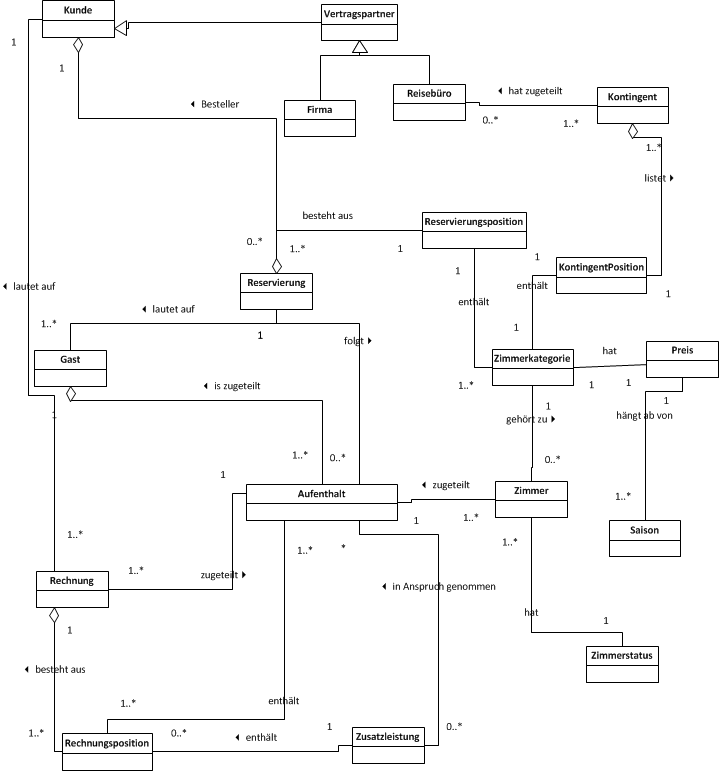
\includegraphics[width=\linewidth]{Images/Domaenenmodell_Uebersicht.png}
\subsection{Detailliertes Modell}
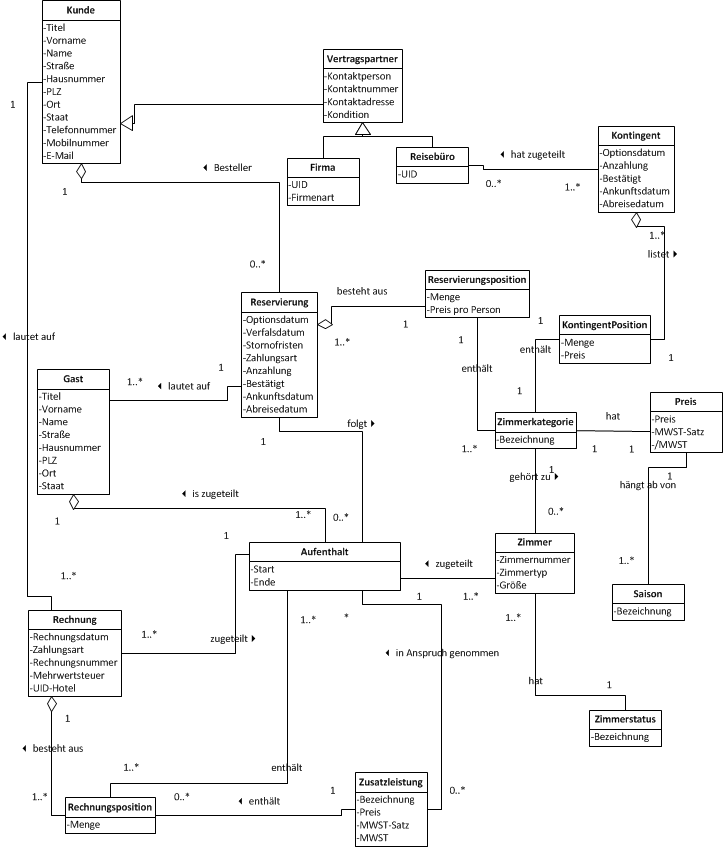
\includegraphics[width=\linewidth]{Images/Domaenenmodell.png}
\subsubsection{Gast}
Beim Gast meint man eine Person welche im Hotel Leistungen bezieht. In ihr ist unter anderem der Name und die Anschrift der Person festgehalten.
\subsubsection{Reservierung}
Eine Reservierung besteht aus verschiedenen Reservierungspositionen, welche eine Zimmerkategorie und eine Menge enthalten. Dazu wird noch der Kunde gespeichert, welcher die Resevierung getätigt hat.
\subsubsection{Reservierungsposition}
Die Reservierungsposition gibt an in welcher Kategorie eine bestimmte Anzahl von
Zimmern reserviert wurde.
\subsubsection{Vertragspartner}
Beim Vertragspartner handelt es sich um eine spezielle Form eines \Gls{Kunde}n.
Er hat einen Vertrag mit dem Hotel abgeschlossen und erhält spezielle Konditionen. Die Vertragspartner werden unterteilt in Firmen und \Glspl{Reisebuero}.
\subsubsection{Firma}
Eine Firma ist ein spezieller Vertragspartner, sie erhält spezielle Konditionen
durch den Vertrag den sie abgeschlossen hat.
\subsubsection{Reisebüro}
Eine Firma ist ein spezieller Vertragspartner, durch den Vertrag der
abgeschlossen wurde kann ein \Gls{Reisebuero} ein bestimmtes Kontingent
zugewiesen bekommen.
\subsubsection{Kontingent}
Bei dem Kontingent handelt es sich um eine spezielle Art von Reservierung die nur für \Glspl{Reisebuero} verwendet werden. Für sie gelten spezielle Regelungen und werden deshalb getrennt verwaltet.
\subsubsection{Kontingentposition}
Eine Kontingentposition ist eine Aufzählung von Zimmern einer bestimmten
Kategorie. Sie ist einem Kontingent zugewiesen.
\subsubsection{Zimmer}
Das Hotelzimmer ist ein Raum den ein Kunde gegen Bezahlung in Anspruch nehmen kann.
\subsubsection{Zimmerstatus}
Der Zimmerstatus beschreibt in welcher Lage sich das Zimmer im aktuellen Moment befindet.
\subsubsection{Zimmerkategorie}
Die Zimmer werden in bestimmte Kategorien unterteilt. Von jeder Kategorie ist
nur eine bestimmte Anzahl von Zimmern vorhanden, welche auch einen Preis
zugewiesen haben.
\subsubsection{Kunde}
Der Kunde ist die Instanz die in direkten Zusammenhang mit einer Rechnung steht.
Einem Kunden ist eindeutig eine Rechnung zuzuordnen.
\subsubsection{Rechnung}
Eine Rechnung wird erstellt und durch ein Zahlungsmittel beglichen, dann gilt die Rechnung als abgeschlossen. Eine Rechnung hat folgende Bestandteile.
\subsubsection{Rechnungsposition}
Die Rechnungsposition enthält die Anzahl einer bestimmten Zusatzleistung oder
eines Aufenthaltes. Sie wird in einer Rechnung aufgelistet.
\subsubsection{Preis}
Der Preis gibt an wie viel ein Zimmer in einer bestimmten Kategorie kostet. Er
ist unter anderem abhängig von der Saison.
\subsubsection{Saison}
Da es verschiedene Saisonen im Jahr gibt, wird mit dieser Saison angegeben
welcher Einfluss auf den Preis etc genommen wird. 
\subsubsection{Aufenthalt}
Der Aufenthalt gibt an welcher bzw. welche Gast bzw Gäste welche Zimmer haben.
Außerdem wird dem Aufenthalt die Zusatzleistungen zugewiesen. Der Aufenthalt ist
auch eine eigene Rechnungsposition.
\subsubsection{Zusatzleistung}
Bei einer Zusatzleistung handelt es sich um eine bestimmte Leistung welche nicht
beim normalen Aufenthalt inkludiert ist. Sie wird zusätzlich verrechnet.

\newpage

\section{Dynamisches Modell}
\subsection{Detaillierte Benutzungsfallbeschreibungen}
\input UseCases/checkin_walkin
\input UseCases/checkin_reisegruppe
\input UseCases/checkin_reservierung
\input UseCases/checkout
\input UseCases/reservierung_firmen
\input UseCases/reservierung_individualgast
\input UseCases/reservierung_reisebuero
\input UseCases/reservierung_aendern
\input UseCases/reservierung_bestaetigen
\input UseCases/reservierung_stornieren_individualperson
\input UseCases/reservierung_stornieren_vertragspartner
\input UseCases/aufenthalt_verlaengern
\input UseCases/zimmer_wechsel
\input UseCases/zimmerstammdaten

\newpage

\section{Nichtfunktionale Anforderungen}
\subsection{Usability}
Natürlich wird versucht die Software selbsterklärend zu gestalten, trotzdem inkludiert das Projekt eine fortlaufende Dokumentation, sowie eine Hilfe, die die Einarbeitungszeit wesentlich verringern soll.

Weiters soll die Software über eine flache Lernkurve verfügen, und somit wenig Schulungsaufwand erzeugen. Das soll durch das Verwenden von bereits bekannten mentalen Modellen und Design Patterns, welche auch in anderer gängiger Software zum Einsatz kommen, erreicht werden.
\subsection{Zuverlässigkeit}
Die Datenbank, auf der das System arbeitet, sollte sich immer einen konsistenten Zustand merken, damit im Fehlerfall ein einfacher Neustart des Systems zur Behebung ausreicht. Trotzdem sollten am besten noch automatisiert Backups erstellt werden, um die Wahrscheinlichkeit eines zu großen Datenverlusts zu begrenzen.
\subsection{Performanz}
Es ist für die Zufriedenheit des Kunden, und somit auch für den \Gls{Rezeptionist}, äußerst wichtig dass oft vorkommende Tätigkeiten schnell abgehandelt werden können. Dazu zählen vor allem der \Gls{Checkin}, und der \Gls{Checkout}, welche, insofern keine Daten nachzutragen bzw. andere Zusatzaufwände zu erledigen sind, nicht länger als 2 Minuten dauern sollten.

Außerdem ist die ständige Verfügbarkeit des Systems von großer Bedeutung, damit Anfragen von Kunden bzw. Gästen sofort bearbeitet werden können. Sollte die Verfügbarkeit für einen gewissen Zeitraum nicht gegeben sein, z.B. wegen Wartungsarbeiten, dann muss dieser Ausfall bereits im Vorherein kommuniziert werden, sodass das Persoal sich auf diese unangenehme Situation vorbereiten kann.
\subsection{Unterstützbarkeit}
Um eine möglichst breite Benutzerschaft anzusprechen, wird die Software mehrsprachig gehalten. Leider können wir aus Zeitgründen nicht auf Seh- oder andere Behinderungen eingehen, so dass eingeschränkte Personen auf andere Hilfsmittel wie Screenreader oder ähnliches zurückgreifen müssen.

Das Verwenden einer Maus soll aber schon optional sein, da die Einstiegshürde andernfalls für Menschen mit Sehbehinderung außerordentlich groß wäre. Das heißt dass die Software auch alleine mit der Tastatur zu bedienen sein sollte.
\subsection{Schnittstellen}
\subsubsection{Benutzerschnittstellen}
Die Software wird vom Benutzer über eine grafische Benutzeroberfläche auf handelsüblichen Desktoprechnern bedient.

Das Hauptfenster soll die Grundfunktionalitäten (Reservierungen, Gäste, ...) über einzelne Reiter zur Verfügung stellen. Die Auflistung dieser Elemente erfolgt über Listen, wobei das aktuell ausgewählte Element in einer Vorschau auch editiert werden kann. Über diverse Buttons können verschiedene Aktionen gestartet werden.

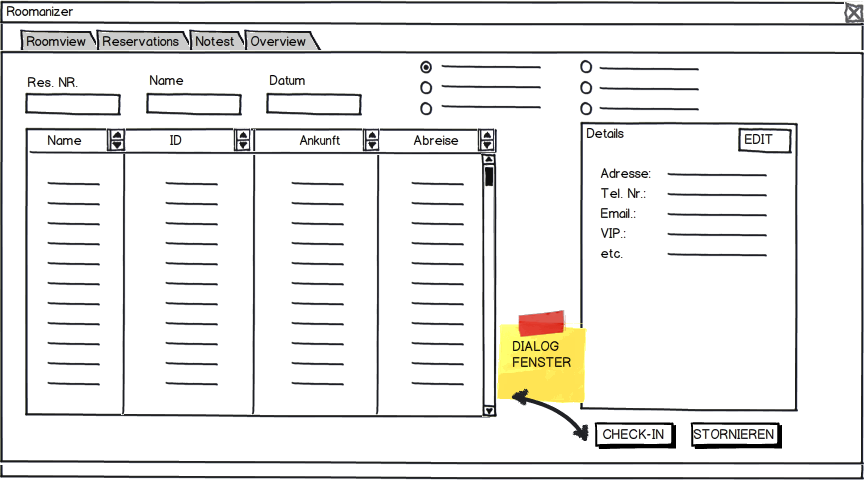
\includegraphics[width=\linewidth]{Images/GUI_Overview.png}

Als kurzes Beispiel sei hier noch ein der Umgang mit Reservierungen erwähnt. Wie bereits erwähnt enthält ein Tab eine Liste mit allen Reservierungen. Bei Auswahl einer Reservierung sieht man rechts eine editierbare Vorschau, und einige Buttons, mit denen man Aktionen auf Bezug des aktuell ausgewählten Element auswählen kann.

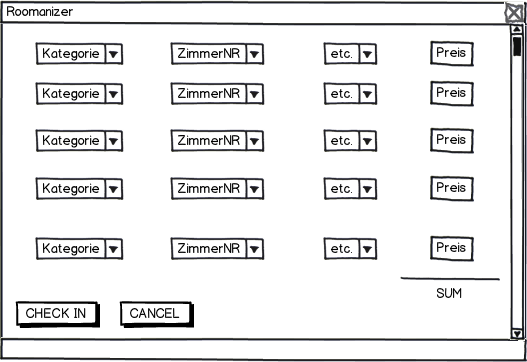
\includegraphics[width=\linewidth]{Images/GUI_Dialog.png}

Drückt man z.B. den Checkin-Button, so erhält man ein Dialogfenster, in dem man eine Auflistung aller zugewiesenen Zimmer, und deren Preise hat. All diese Informationen können noch geändert werden, bevor man mit einem Klick die ganzen Zimmer vergibt.
\subsubsection{Software Schnittstellen}
Es sind Schnittstellen zu den bestehenden Systemen (Finanzbuchhaltung, Debitorenbuchhaltung, Food and Beverage Verwaltung) vorzusehen.
\subsubsection{Kommunikationsschnittstellen}
Es ist nicht vorgesehen, dass das System von jedem Mitarbeiter des Hotels zu bedienen ist, da es gerade bei Mitarbeiter in Positionen mit hoher Fluktuation zu teuer wäre, jeden einzelnen dem Umgang mit der Software zu erläutern. Daher werden immer noch diverse Formulare existieren, die von gewissen Berufsgruppen (z.B. Reinigungspersonal) ausgefüllt, und danach von Mitarbeitern im Backoffice manuell ins System übertragen werden.

\newpage

\section{Iterationsplan (Timeboxes)}
\input iterationsplan

\newpage

%Glossar
\addcontentsline{toc}{section}{Glossar}
\printglossary[title=Glossar,toctitle=GLOSSAR]
\end{document}
